%% LyX 2.3.6 created this file.  For more info, see http://www.lyx.org/.
%% Do not edit unless you really know what you are doing.
\documentclass[english,aspectratio=169]{beamer}
\usepackage{lmodern}
\renewcommand{\sfdefault}{lmss}
\renewcommand{\ttdefault}{lmtt}
\usepackage[T1]{fontenc}
\usepackage[latin9]{inputenc}
\setlength{\parskip}{\medskipamount}
\setlength{\parindent}{0pt}
\usepackage{amssymb}
\usepackage{graphicx}

\makeatletter

%%%%%%%%%%%%%%%%%%%%%%%%%%%%%% LyX specific LaTeX commands.
\pdfpageheight\paperheight
\pdfpagewidth\paperwidth

%% Because html converters don't know tabularnewline
\providecommand{\tabularnewline}{\\}

%%%%%%%%%%%%%%%%%%%%%%%%%%%%%% Textclass specific LaTeX commands.
% this default might be overridden by plain title style
\newcommand\makebeamertitle{\frame{\maketitle}}%
% (ERT) argument for the TOC
\AtBeginDocument{%
  \let\origtableofcontents=\tableofcontents
  \def\tableofcontents{\@ifnextchar[{\origtableofcontents}{\gobbletableofcontents}}
  \def\gobbletableofcontents#1{\origtableofcontents}
}

%%%%%%%%%%%%%%%%%%%%%%%%%%%%%% User specified LaTeX commands.
\usetheme{CambridgeUS}
\usecolortheme{dolphin}
\hypersetup{}
\usepackage{tikz}
\usepackage{color}
\usepackage{listings}

\makeatother

\usepackage{babel}
\begin{document}
\title[M3-6]{The geostrophic balance and the Rossby number}
\author{Department of Oceanography}
\institute[UCT]{University of Cape Town}
\date{SEA3004F}
\makebeamertitle

\section*{Outlines}
\begin{frame}{Outline}

\tableofcontents{}
\end{frame}


\section{Balanced circulation}
\begin{frame}{Patterns of the general circulation }

\begin{columns}[t]


\column{7 cm}
\begin{itemize}
\item Every large scale permanent feature we see must be due to a balance
between all the governing forces, otherwise it would not be permanent
but transient
\item An analysis of the mean wind circulation shows a seasonal variability,
but the wind tends to flow around the centres of high and low pressure
with clear patterns
\end{itemize}

\column{7 cm}

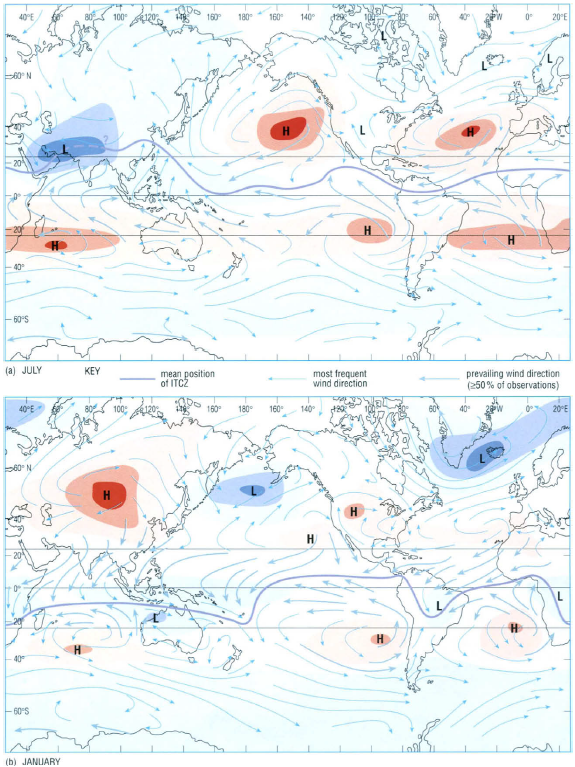
\includegraphics[height=0.7\paperheight]{figures/M3/circulation_patterns_high-low}
\end{columns}

\end{frame}

\begin{frame}{An empirical law for synoptic circulation}

\begin{columns}[t]


\column{8 cm}
\begin{itemize}
\item {\footnotesize{}Even when the circulation is transient, as in the
case of synoptic weather chart shown here, we can still see the emergence
of major patterns in the flow: the wind follows isobars }\textbf{\footnotesize{}in
some predictable way}{\footnotesize\par}
\item {\footnotesize{}This was initially deduced through empirical observations
by the Dutch meteorologist Buys-Ballot and became known as the Buys-Ballot
law (Academie des sciences. Comptes rendus hebdomadaires, TOME XLV,
JUILLET - DECEMBRE (1857) pp. 765\textendash 768)}{\footnotesize\par}
\end{itemize}
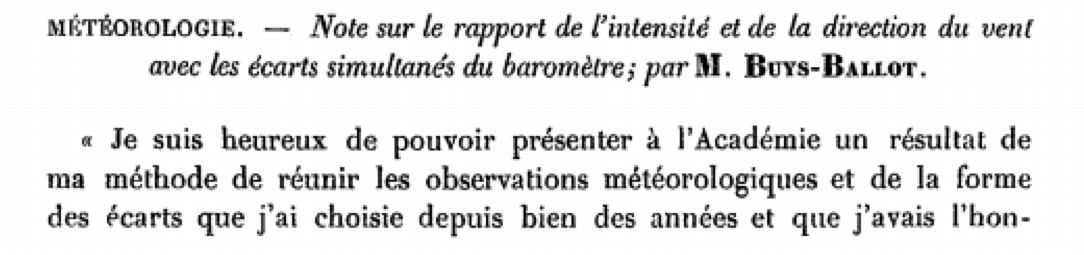
\includegraphics[scale=0.4]{figures/M3/buy-ballot}

\column{5 cm}

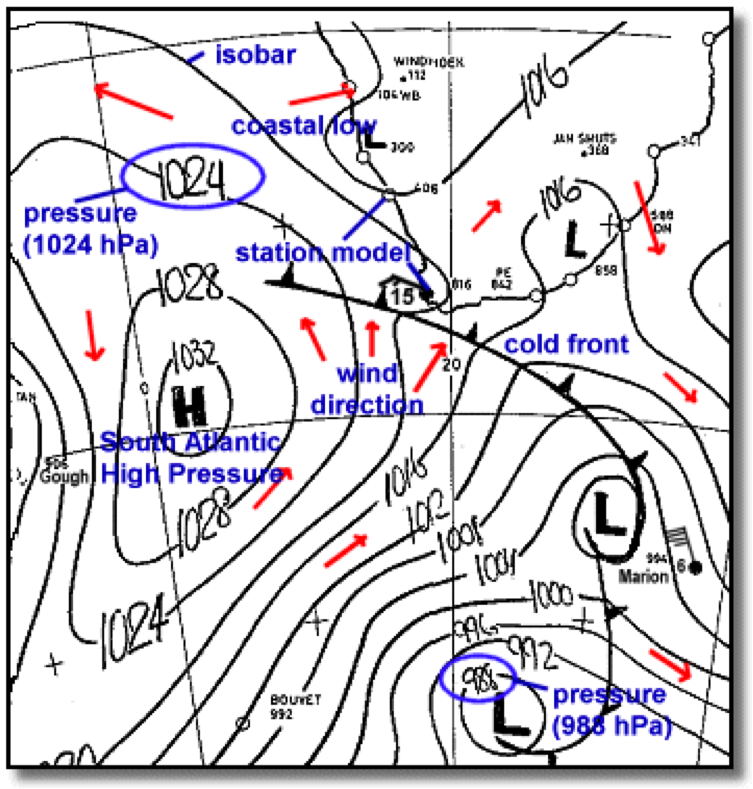
\includegraphics[width=5cm]{figures/M3/synoptic_chart}
\end{columns}

\end{frame}

\begin{frame}{Major balances in geophysical flows}

\begin{itemize}
\item In this lecture we will manipulate the Navier-Stokes equation to explain
why such major patterns emerge from the complex behavior of geophysical
fluids
\item To do this, we need to understand the concept of \textbf{dimensional
analysis}, a fundamental methods in physics and engineering that allows
us to gain insights on dynamical processes by looking at their typical
temporal and spatial scales. Through dimensional analysis, equations
can be rearranged in such a way to reveal major properties that are
somewhat hidden
\item This method was applied to meteorology by one of the most influential
scientists in the field, C-G Rossby
\end{itemize}
\end{frame}

\begin{frame}{The weather man: Rossby}

\begin{columns}[t]


\column{4cm}

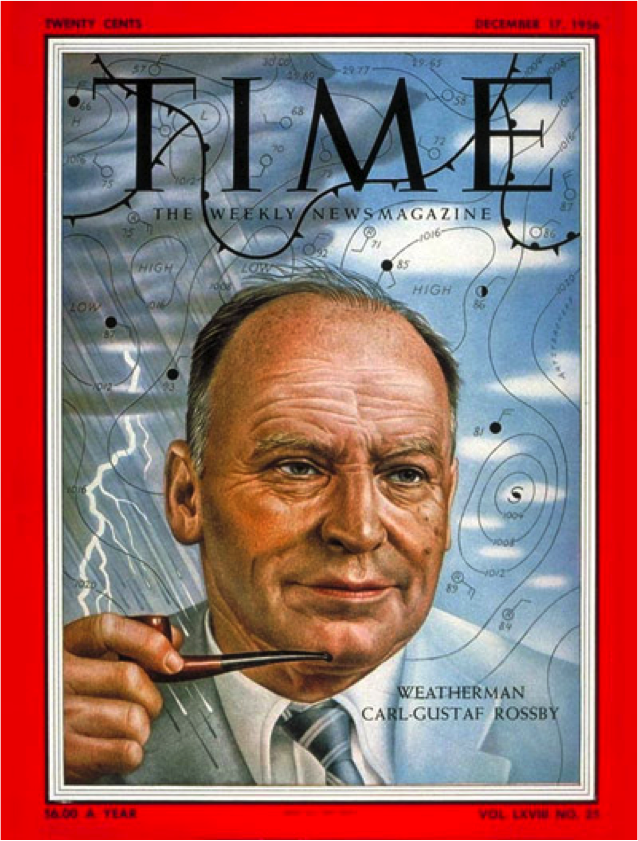
\includegraphics[width=4cm]{figures/M3/rossby}

\column{9cm}
\begin{itemize}
\item \textbf{\small{}Carl-Gustaf Arvid Rossby 1898 \textendash{} 1957}{\small{}
A Swedish meteorologist, Carl-Gustav Rossby is credited with most
of the fundamental principles on which geophysical fluid dynamics
rests. Among other contributions, he left us the concepts of radius
of deformation, planetary waves, and geostrophic adjustment. }\emph{\small{}Note:
the dimensionless number that bears his name was first introduced
by the Soviet scientist I. A. Kibel\textquoteright{} in 1940.}{\small\par}
\item {\small{}During a number of years spent in the United States, he established
the meteorology departments at MIT and the University of Chicago.
He later returned to his native Sweden to become the director of the
Institute of Meteorology in Stockholm. }\emph{\small{}(I met his son!...
sorry, could not resist to tell you...)}{\small\par}
\end{itemize}
\end{columns}

\end{frame}


\section{Dimensional analysis}
\begin{frame}{Dimensional analysis}

\begin{itemize}
\item {\small{}In dimensional analysis we assume that every quantity can
be written in terms of a typical value that is characteristic of the
process }{\small\par}
\item {\small{}For instance, the typical length scale of an ocean basin
is ``of order'' 1000 km. This does not mean that all basins must
have this size but that in general the Atlantic Ocean, or the Pacific
Ocean are measurable in multiples of 1000 km. An upwelling system,
on the other hand, would be measured in multiples of 100 km. If we
call $L$ the characteristic length scale, then the spatial variable
$x$ can be written as 
\[
x=L\,x^{*}
\]
where $x^{*}$ is a non-dimensional variable constrained within a
given range that is realistic enough. Similarly, the speed of a major
current system $\left(u=Uu^{*}\right)$ will be a fraction or a multiple
of $U$, which gives the order of magnitude of the flow velocity.
You can also think of $U$ as the mean speed and $u^{*}$ are the
relative fluctuations around the mean}{\small\par}
\item {\small{}We can apply this principle to all the spatial and temporal
scales in the ocean and the atmosphere using the values shown in the
next table}{\small\par}
\end{itemize}
\end{frame}

\begin{frame}{Orders of magnitude of synoptic processes}

\begin{table}
\begin{centering}
\begin{tabular}{|l|c|c|c|c|}
\hline 
\textbf{\footnotesize{}Property} & \textbf{\footnotesize{}Symbol} & \textbf{\footnotesize{}Atmosphere} & \textbf{\footnotesize{}Ocean} & \textbf{\footnotesize{}Units}\tabularnewline
\hline 
\hline 
{\footnotesize{}Horizontal scale} & {\footnotesize{}$L$} & {\footnotesize{}$10^{6}$} & {\footnotesize{}$10^{6}$} & {\footnotesize{}m}\tabularnewline
\hline 
{\footnotesize{}Time scale} & {\footnotesize{}$T$} & {\footnotesize{}$10^{5}$ (day)} & {\footnotesize{}$10^{6}$ (week)} & {\footnotesize{}s}\tabularnewline
\hline 
{\footnotesize{}Vertical scale} & {\footnotesize{}$H$} & {\footnotesize{}$10^{4}$} & {\footnotesize{}$10^{3}$} & {\footnotesize{}m}\tabularnewline
\hline 
{\footnotesize{}Horizontal velocity} & {\footnotesize{}$U$} & {\footnotesize{}$10$} & {\footnotesize{}$10^{-1}$} & {\footnotesize{}m s$^{-1}$}\tabularnewline
\hline 
{\footnotesize{}Vertical velocity} & {\footnotesize{}$W$} & {\footnotesize{}$10^{-2}$} & {\footnotesize{}$10^{-5}$} & {\footnotesize{}m s$^{-1}$}\tabularnewline
\hline 
{\footnotesize{}Sea level pressure} & {\footnotesize{}$P$} & {\footnotesize{}$10^{5}$} & {\footnotesize{}$10^{5}$} & {\footnotesize{}Pa}\tabularnewline
\hline 
{\footnotesize{}Pressure fluctuations} & {\footnotesize{}$\Delta P$} & {\footnotesize{}$10^{3}$} & {\footnotesize{}Large} & {\footnotesize{}Pa}\tabularnewline
\hline 
{\footnotesize{}Density} & {\footnotesize{}$\rho_{0}$} & {\footnotesize{}$1$} & {\footnotesize{}$10^{3}$} & {\footnotesize{}kg m$^{-3}$}\tabularnewline
\hline 
{\footnotesize{}Density fluctuations} & {\footnotesize{}$\Delta\rho/\rho$} & {\footnotesize{}$10^{-2}$} & {\footnotesize{}$10^{-3}$} & {\footnotesize{}kg m$^{-3}$}\tabularnewline
\hline 
{\footnotesize{}Pot. temperature fluctuations} & {\footnotesize{}$\Delta\Theta$} & {\footnotesize{}$4$} & {\footnotesize{}Large} & {\footnotesize{}$^{\circ}$C}\tabularnewline
\hline 
{\footnotesize{}Coriolis parameter (mid-latitude)} & {\footnotesize{}$f$} & {\footnotesize{}$10^{-4}$} & {\footnotesize{}$10^{-4}$} & {\footnotesize{}s$^{-1}$}\tabularnewline
\hline 
{\footnotesize{}Viscosity} & {\footnotesize{}$\nu$} & {\footnotesize{}$10^{-5}$} & {\footnotesize{}$10^{-6}$} & {\footnotesize{}m$^{2}$s$^{-1}$}\tabularnewline
\hline 
\end{tabular}
\par\end{centering}
\caption{Typical synoptic scales in the ocean and in the atmosphere, and typical
parameter values}
\end{table}

\end{frame}

\begin{frame}{Dimensional analysis of the equation of motion}

\begin{itemize}
\item {\small{}Let's start from the }\textbf{\small{}horizontal components}{\small{}
of the Navier-Stokes $\vec{u_{H}}=\left\langle u,v\right\rangle $}
\begin{align*}
\frac{\partial u}{\partial t}+u\frac{\partial u}{\partial x}+v\frac{\partial u}{\partial y}+w\frac{\partial u}{\partial z} & -fv=-\frac{1}{\rho}\frac{\partial p}{\partial x}+\nu\left(\frac{\partial^{2}u}{\partial x^{2}}+\frac{\partial^{2}u}{\partial y^{2}}+\frac{\partial^{2}u}{\partial z^{2}}\right)\\
\frac{\partial v}{\partial t}+u\frac{\partial v}{\partial x}+v\frac{\partial v}{\partial y}+w\frac{\partial v}{\partial z} & +fu=-\frac{1}{\rho}\frac{\partial p}{\partial y}+\nu\left(\frac{\partial^{2}v}{\partial x^{2}}+\frac{\partial^{2}v}{\partial y^{2}}+\frac{\partial^{2}v}{\partial z^{2}}\right)
\end{align*}
\item {\small{}We apply a dimensional analysis for the atmosphere and the
ocean using the previous table. Note that changes are assumed to have
the same order of magnitude of the quantity, like $\Delta u\approx U$,
$\Delta t\approx T$, except when they are known to be smaller, like
with density in the ocean.}{\small\par}
\end{itemize}
\begin{center}
\begin{tabular}{|c|c|c|c|c|c|c|c|}
\hline 
{\scriptsize{}Terms} & {\scriptsize{}$\frac{\partial u}{\partial t}$} & {\scriptsize{}$u\frac{\partial u}{\partial x}$} & {\scriptsize{}$v\frac{\partial u}{\partial x}$} & {\scriptsize{}$w\frac{\partial u}{\partial z}$} & {\scriptsize{}$fv$} & {\scriptsize{}$\frac{1}{\rho}\frac{\partial p}{\partial x}$} & {\scriptsize{}$\nu\frac{\partial^{2}u}{\partial x^{2}}$}\tabularnewline
\hline 
{\scriptsize{}Symbols} & {\scriptsize{}$\frac{U}{T}$} & {\scriptsize{}$\frac{U^{2}}{L}$} & {\scriptsize{}$\frac{U^{2}}{L}$} & {\scriptsize{}$\frac{WU}{H}$} & {\scriptsize{}$fU$} & {\scriptsize{}$\frac{\Delta P}{\rho L}$} & {\scriptsize{}$\nu\frac{U}{L^{2}}$}\tabularnewline
\hline 
{\scriptsize{}Atmosphere} & {\tiny{}$\frac{10}{10^{5}}$} & {\tiny{}$\frac{10\cdot10}{10^{6}}$} & {\tiny{}$\frac{10^{2}}{10^{6}}$} & {\tiny{}$\frac{10^{-2}\cdot10}{10^{4}}$} & {\tiny{}$10^{-4}\cdot10$} & {\tiny{}$\frac{10^{3}}{1\cdot10^{6}}$} & {\tiny{}$\frac{10^{-5}\cdot10}{10^{6}\cdot10^{6}}$}\tabularnewline
\hline 
{\scriptsize{}Ocean} & {\tiny{}$\frac{10^{-1}}{10^{6}}$} & {\tiny{}$\frac{10^{-1}\cdot10^{-1}}{10^{6}}$} & {\tiny{}$\frac{10^{-2}}{10^{6}}$} & {\tiny{}$\frac{10^{-5}\cdot10^{-1}}{10^{3}}$} & {\tiny{}$10^{-4}\cdot10^{-1}$} & {\tiny{}$\frac{?}{10^{3}\cdot10^{6}}$} & {\tiny{}$\frac{10^{-6}\cdot10^{-1}}{10^{6}\cdot10^{6}}$}\tabularnewline
\hline 
\end{tabular}
\par\end{center}

\end{frame}

\begin{frame}{A non-dimensional equation of motion}

\begin{itemize}
\item {\small{}It is no accident that }\textbf{\small{}the local acceleration
term}{\small{} $\frac{\partial\mathbf{u}}{\partial t}$ and }\textbf{\small{}the
momentum advection term}{\small{} $\mathbf{u}\cdot\nabla\mathbf{u}$
}\textbf{\small{}are comparable in magnitude}{\small{}, especially
in the atmosphere: the timescale on which motions change is related
to the time taken for the flow to traverse a distance $L$. This means
that $U/T=U^{2}/L$ since we can write $T=L/U$}{\small\par}
\item {\small{}We also see from the previous table (clearly in the atmosphere
and very likely in the ocean) that t}\textbf{\small{}he two larger
terms are Coriolis and the pressure gradient accelerations}{\small{}.
(Note that the dimensional analysis can also be done in the vertical
component. In that case the typical ocean pressure gradient is well
known) }{\small\par}
\item {\small{}If we neglect from the beginning the quantities involving
vertical velocities and friction (that are much smaller) and write
$u=Uu^{*}$, so that $u^{*}$ is now a non-dimensional velocity and
we do the same for the other terms ($t=Tt^{*}$, $x=Lx^{*}$ and so
on), we obtain a non-dimensional version of the horizontal momentum
equation
\[
\frac{U^{2}}{L}\left(\frac{\partial\mathbf{u}_{H}^{*}}{\partial t}+\mathbf{u}_{H}^{*}\cdot\nabla_{H}\mathbf{u}_{H}^{*}\right)+fU\hat{\mathbf{k}}\times\mathbf{u}_{H}^{*}=-\frac{\Delta P}{L}\frac{\nabla_{H}p^{*}}{\rho}
\]
where the $H$ subscript stands for the horizontal components $\mathbf{u}_{H}^{*}=\left\langle u^{*},v^{*}\right\rangle $. }{\small\par}
\end{itemize}
\end{frame}

\begin{frame}{The Rossby number}

\begin{itemize}
\item Dividing by $fU$ we see that \textbf{the acceleration terms are scaled
by a typical parameter}, called the \textbf{Rossby number} $\boxed{R_{o}=U/fL}$
\[
R_{o}\left(\frac{\partial\mathbf{u}_{H}^{*}}{\partial t}+\mathbf{u}_{H}^{*}\cdot\nabla_{H}\mathbf{u}_{H}^{*}\right)+\hat{\mathbf{k}}\times\mathbf{u}_{H}^{*}=-\frac{\Delta P}{fUL}\frac{\nabla_{H}p^{*}}{\rho}
\]
\item The value of the Rossby number in the atmosphere is $10/\left(10^{-4}\cdot10^{6}\right)=0.1$
and in the ocean is even smaller, so the terms that are multiplied
by it can be neglected. \textbf{The major balance at the larger scales
is achieved between Coriolis and the pressure gradient}
\end{itemize}
\end{frame}


\section{The geostrophic balance}
\begin{frame}{The geostrophic flow}

\begin{columns}[t]


\column{7.5cm}
\begin{itemize}
\item {\scriptsize{}When the fluid is set into motion because of a pressure
gradient force, it is affected by the Coriolis force that tends to
veer it on a side (right in the NE, left in the SE). In the figure,
the pressure gradient is indicated by the elevation of the ocean surface
towards the East.}{\scriptsize\par}
\item {\scriptsize{}The fluid will be deviated until the two accelerations
are balanced, one against the other, and the flow goes perpendicular
to the acting forces with intensity
\[
V=\frac{1}{\rho f}\frac{\partial p}{\partial x}
\]
}\emph{\scriptsize{}(note: here we are looking at pressure that varies
along the X-axis only. There is also a component along the Y-axis)}{\scriptsize{} }{\scriptsize\par}
\item {\scriptsize{}We call }\textbf{\scriptsize{}geostrophic flow}{\scriptsize{}
(}\emph{\footnotesize{}geo,}{\footnotesize{} Earth and }\emph{\footnotesize{}strophe}{\footnotesize{},
turning}{\scriptsize{}) any motion that is due to a balance between
the pressure gradient and the Coriolis forces}{\scriptsize\par}
\end{itemize}

\column{6cm}
\begin{center}
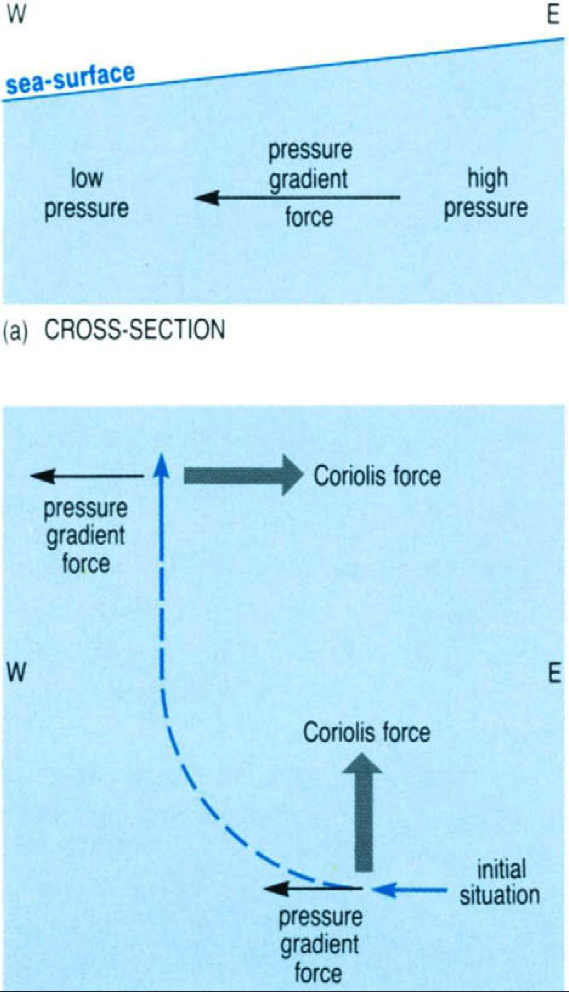
\includegraphics[width=4cm]{figures/M3/geostrophy_OU}
\par\end{center}

\end{columns}

\end{frame}

\begin{frame}{The geostrophic balance}

\begin{center}
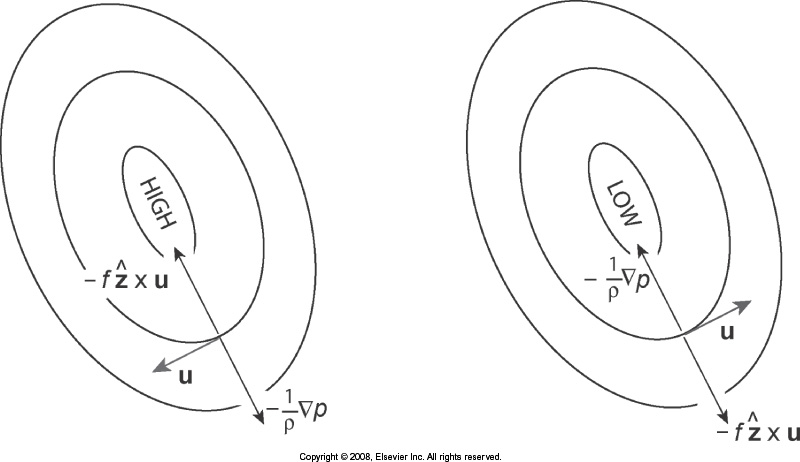
\includegraphics[width=5cm]{figures/M3/f07-01-P558691}
\par\end{center}
\begin{itemize}
\item {\footnotesize{}If we now go back to the dimensional variables of
the Navier-Stokes equations and consider only the dominant terms,
we see the following balance
\[
\boxed{f\left(\hat{\mathbf{k}}\times\mathbf{u}_{H}\right)+\frac{\nabla_{H}p}{\rho_{0}}=0}
\]
}{\footnotesize\par}
\item {\footnotesize{}The }\textbf{\footnotesize{}geostrophic wind or current}{\footnotesize{}
is the velocity field that satisfies the above relationship.}{\footnotesize\par}
\end{itemize}
\end{frame}

\begin{frame}{The geostrophic wind or current}

\begin{center}
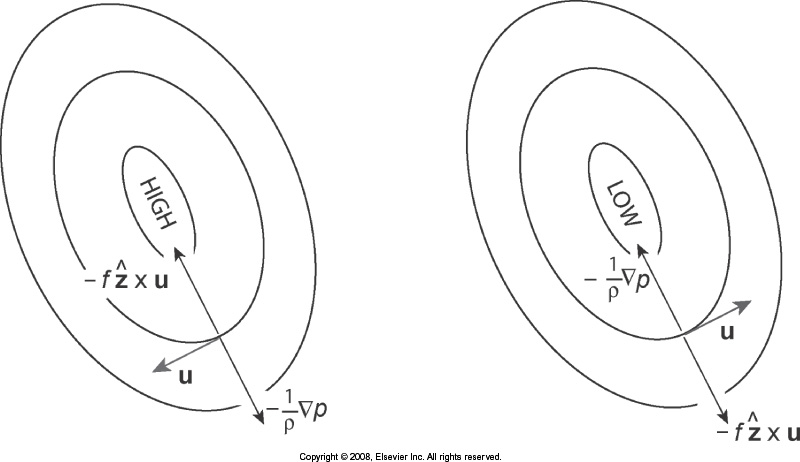
\includegraphics[width=5cm]{figures/M3/f07-01-P558691}
\par\end{center}
\begin{itemize}
\item {\footnotesize{}By noting that $\hat{\mathbf{k}}\times\hat{\mathbf{k}}\times\mathbf{u}=-\mathbf{u}$,
and resolving for $\mathbf{u}$, we obtain the vector formulation
of the geostrophic wind or current, which we call $\mathbf{u}_{g}$:
\[
\boxed{\mathbf{u}_{g}=\frac{1}{f\rho_{0}}\hat{\mathbf{k}}\times\nabla_{H}p;\ \ \left\langle u_{g},v_{g}\right\rangle =\left\langle -\frac{1}{f\rho_{0}}\frac{\partial p}{\partial y},\frac{1}{f\rho_{0}}\frac{\partial p}{\partial x}\right\rangle }
\]
}{\footnotesize\par}
\item {\scriptsize{}It is advised to work out the vector calculus and convince
yourself of this equivalence}{\scriptsize\par}
\item {\scriptsize{}The geostrophic flow is perpendicular to the pressure
gradient in the atmosphere or the sea surface height gradient in the
ocean. It follows the lines of equal pressure (surface height), which
are streamlines of the velocity field. This is a quantitative demonstration
of what was empirically observed by Buys-Ballot and it's a fundamental
property of geophysical fluids}{\scriptsize\par}
\end{itemize}
\end{frame}


\end{document}
